\documentclass{standalone}
\usepackage{tikz}
\usetikzlibrary{patterns, positioning}

\begin{document}
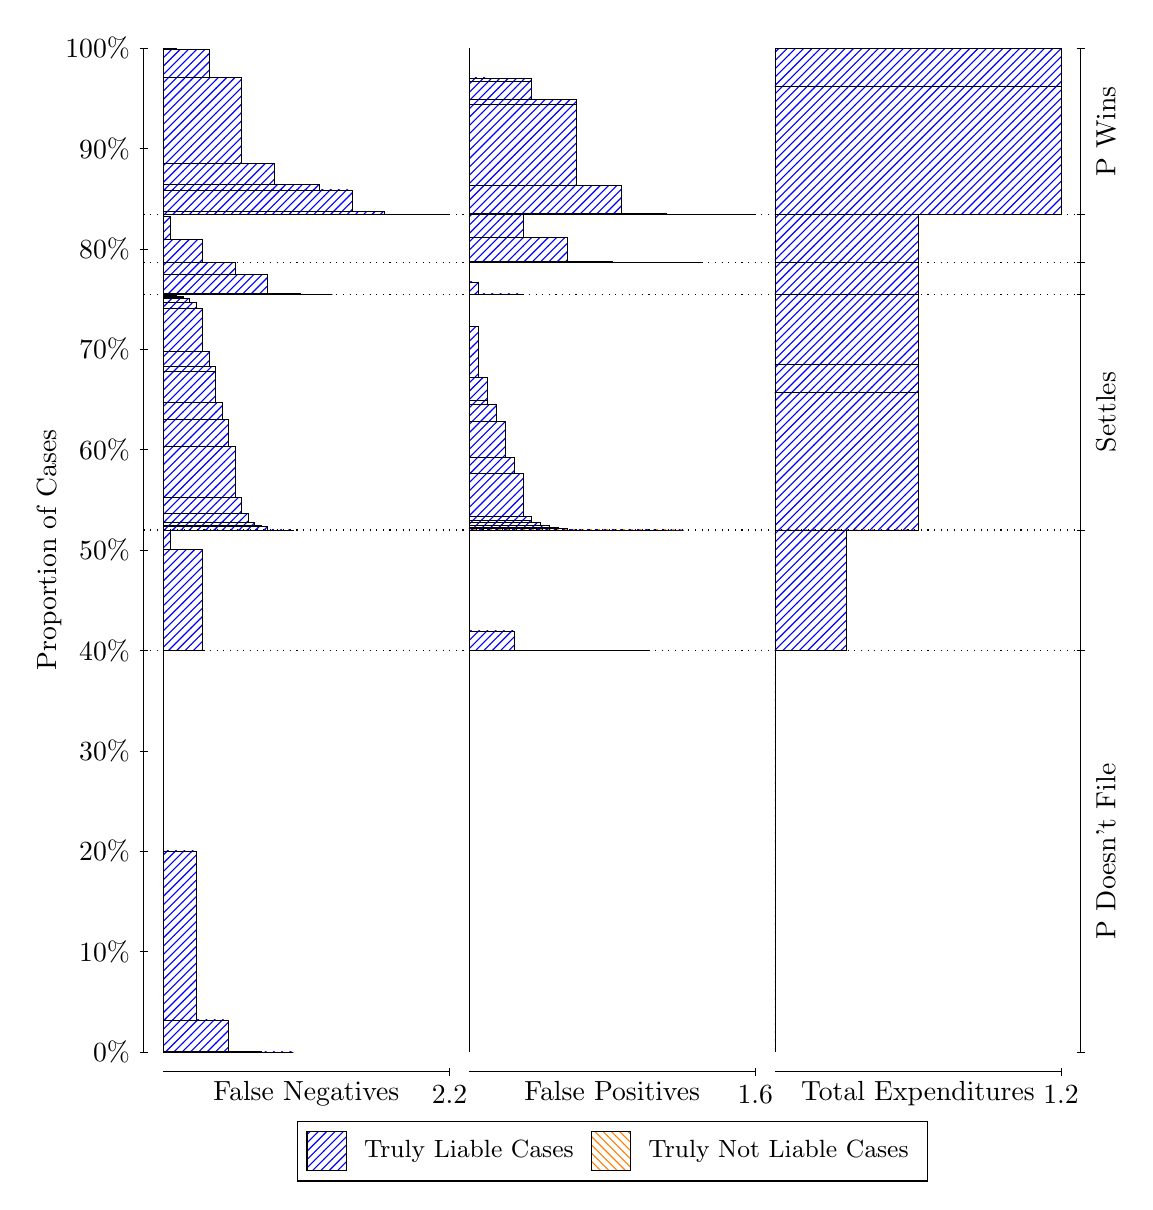
\begin{tikzpicture}
\draw[black, very thin] (1.5,1.75) -- (1.5,14.5);
\node[rotate=90, anchor=center] at (0.3, 8.125) {Proportion of Cases};
\draw[black, very thin] (1.45,1.75) -- (1.55,1.75);
\node[anchor=east] at (1.45, 1.75) {0\%};
\draw[black, very thin] (1.45,3.025) -- (1.55,3.025);
\node[anchor=east] at (1.45, 3.025) {10\%};
\draw[black, very thin] (1.45,4.3) -- (1.55,4.3);
\node[anchor=east] at (1.45, 4.3) {20\%};
\draw[black, very thin] (1.45,5.575) -- (1.55,5.575);
\node[anchor=east] at (1.45, 5.575) {30\%};
\draw[black, very thin] (1.45,6.85) -- (1.55,6.85);
\node[anchor=east] at (1.45, 6.85) {40\%};
\draw[black, very thin] (1.45,8.125) -- (1.55,8.125);
\node[anchor=east] at (1.45, 8.125) {50\%};
\draw[black, very thin] (1.45,9.4) -- (1.55,9.4);
\node[anchor=east] at (1.45, 9.4) {60\%};
\draw[black, very thin] (1.45,10.675) -- (1.55,10.675);
\node[anchor=east] at (1.45, 10.675) {70\%};
\draw[black, very thin] (1.45,11.95) -- (1.55,11.95);
\node[anchor=east] at (1.45, 11.95) {80\%};
\draw[black, very thin] (1.45,13.225) -- (1.55,13.225);
\node[anchor=east] at (1.45, 13.225) {90\%};
\draw[black, very thin] (1.45,14.5) -- (1.55,14.5);
\node[anchor=east] at (1.45, 14.5) {100\%};

\draw[black, very thin] (13.4,1.75) -- (13.4,14.5);
\draw[black, very thin] (13.35,1.75) -- (13.45,1.75);
\node[anchor=west] at (13.35, 1.75) {};
\draw[black, very thin] (13.35,6.8489) -- (13.45,6.8489);
\node[anchor=west] at (13.35, 6.8489) {};
\draw[black, very thin] (13.35,8.3791) -- (13.45,8.3791);
\node[anchor=west] at (13.35, 8.3791) {};
\draw[black, very thin] (13.35,11.375) -- (13.45,11.375);
\node[anchor=west] at (13.35, 11.375) {};
\draw[black, very thin] (13.35,11.778) -- (13.45,11.778);
\node[anchor=west] at (13.35, 11.778) {};
\draw[black, very thin] (13.35,12.384) -- (13.45,12.384);
\node[anchor=west] at (13.35, 12.384) {};
\draw[black, very thin] (13.35,14.5) -- (13.45,14.5);
\node[anchor=west] at (13.35, 14.5) {};

\draw[black, very thin, pattern color=blue, pattern=north east lines] (1.75,1.75) rectangle (3.4015,1.75);
\draw[black, very thin, pattern color=blue, pattern=north east lines] (1.75,1.75) rectangle (2.9886,1.7534);
\draw[black, very thin, pattern color=blue, pattern=north east lines] (1.75,1.7534) rectangle (2.5758,2.158);
\draw[black, very thin, pattern color=blue, pattern=north east lines] (1.75,2.158) rectangle (2.1629,4.3029);
\draw[black, very thin, pattern color=orange, pattern=north west lines] (1.75,4.3029) rectangle (1.75,4.3029);
\draw[black, very thin, pattern color=blue, pattern=north east lines] (1.75,4.3029) rectangle (1.75,6.8489);
\draw[black, very thin, pattern color=blue, pattern=north east lines] (1.75,6.8489) rectangle (2.2455,8.1291);
\draw[black, very thin, pattern color=blue, pattern=north east lines] (1.75,8.1291) rectangle (1.8326,8.3773);
\draw[black, very thin, pattern color=orange, pattern=north west lines] (1.75,8.3773) rectangle (1.75,8.3773);
\draw[black, very thin, pattern color=blue, pattern=north east lines] (1.75,8.3773) rectangle (1.75,8.3791);
\draw[black, very thin, pattern color=blue, pattern=north east lines] (1.75,8.3791) rectangle (3.4015,8.3792);
\draw[black, very thin, pattern color=blue, pattern=north east lines] (1.75,8.3792) rectangle (3.2364,8.3795);
\draw[black, very thin, pattern color=blue, pattern=north east lines] (1.75,8.3795) rectangle (3.0712,8.4229);
\draw[black, very thin, pattern color=blue, pattern=north east lines] (1.75,8.4229) rectangle (2.9886,8.441);
\draw[black, very thin, pattern color=blue, pattern=north east lines] (1.75,8.441) rectangle (2.9061,8.4811);
\draw[black, very thin, pattern color=blue, pattern=north east lines] (1.75,8.4811) rectangle (2.8235,8.5913);
\draw[black, very thin, pattern color=blue, pattern=north east lines] (1.75,8.5913) rectangle (2.7409,8.7934);
\draw[black, very thin, pattern color=blue, pattern=north east lines] (1.75,8.7934) rectangle (2.6583,9.4384);
\draw[black, very thin, pattern color=blue, pattern=north east lines] (1.75,9.4384) rectangle (2.5758,9.7812);
\draw[black, very thin, pattern color=blue, pattern=north east lines] (1.75,9.7812) rectangle (2.4932,9.995);
\draw[black, very thin, pattern color=blue, pattern=north east lines] (1.75,9.995) rectangle (2.4106,10.396);
\draw[black, very thin, pattern color=blue, pattern=north east lines] (1.75,10.396) rectangle (2.4106,10.453);
\draw[black, very thin, pattern color=blue, pattern=north east lines] (1.75,10.453) rectangle (2.328,10.651);
\draw[black, very thin, pattern color=blue, pattern=north east lines] (1.75,10.651) rectangle (2.2455,11.2);
\draw[black, very thin, pattern color=blue, pattern=north east lines] (1.75,11.2) rectangle (2.1629,11.274);
\draw[black, very thin, pattern color=blue, pattern=north east lines] (1.75,11.274) rectangle (2.0803,11.32);
\draw[black, very thin, pattern color=blue, pattern=north east lines] (1.75,11.32) rectangle (1.9977,11.337);
\draw[black, very thin, pattern color=blue, pattern=north east lines] (1.75,11.337) rectangle (1.9977,11.346);
\draw[black, very thin, pattern color=blue, pattern=north east lines] (1.75,11.346) rectangle (1.9152,11.356);
\draw[black, very thin, pattern color=blue, pattern=north east lines] (1.75,11.356) rectangle (1.8326,11.374);
\draw[black, very thin, pattern color=orange, pattern=north west lines] (1.75,11.374) rectangle (1.75,11.374);
\draw[black, very thin, pattern color=blue, pattern=north east lines] (1.75,11.374) rectangle (1.75,11.375);
\draw[black, very thin, pattern color=blue, pattern=north east lines] (1.75,11.375) rectangle (3.897,11.375);
\draw[black, very thin, pattern color=blue, pattern=north east lines] (1.75,11.375) rectangle (3.4841,11.386);
\draw[black, very thin, pattern color=blue, pattern=north east lines] (1.75,11.386) rectangle (3.0712,11.623);
\draw[black, very thin, pattern color=blue, pattern=north east lines] (1.75,11.623) rectangle (2.6583,11.776);
\draw[black, very thin, pattern color=blue, pattern=north east lines] (1.75,11.776) rectangle (2.2455,11.778);
\draw[black, very thin, pattern color=orange, pattern=north west lines] (1.75,11.778) rectangle (1.75,11.778);
\draw[black, very thin, pattern color=blue, pattern=north east lines] (1.75,11.778) rectangle (2.2455,12.07);
\draw[black, very thin, pattern color=blue, pattern=north east lines] (1.75,12.07) rectangle (1.8326,12.367);
\draw[black, very thin, pattern color=orange, pattern=north west lines] (1.75,12.367) rectangle (1.75,12.367);
\draw[black, very thin, pattern color=blue, pattern=north east lines] (1.75,12.367) rectangle (1.75,12.384);
\draw[black, very thin, pattern color=blue, pattern=north east lines] (1.75,12.384) rectangle (5.3833,12.384);
\draw[black, very thin, pattern color=blue, pattern=north east lines] (1.75,12.384) rectangle (4.9705,12.385);
\draw[black, very thin, pattern color=blue, pattern=north east lines] (1.75,12.385) rectangle (4.5576,12.428);
\draw[black, very thin, pattern color=blue, pattern=north east lines] (1.75,12.428) rectangle (4.1447,12.699);
\draw[black, very thin, pattern color=blue, pattern=north east lines] (1.75,12.699) rectangle (3.9795,12.699);
\draw[black, very thin, pattern color=blue, pattern=north east lines] (1.75,12.699) rectangle (3.7318,12.764);
\draw[black, very thin, pattern color=blue, pattern=north east lines] (1.75,12.764) rectangle (3.5667,12.769);
\draw[black, very thin, pattern color=blue, pattern=north east lines] (1.75,12.769) rectangle (3.3189,12.769);
\draw[black, very thin, pattern color=blue, pattern=north east lines] (1.75,12.769) rectangle (3.1538,13.034);
\draw[black, very thin, pattern color=blue, pattern=north east lines] (1.75,13.034) rectangle (2.9061,13.034);
\draw[black, very thin, pattern color=blue, pattern=north east lines] (1.75,13.034) rectangle (2.7409,14.124);
\draw[black, very thin, pattern color=blue, pattern=north east lines] (1.75,14.124) rectangle (2.328,14.483);
\draw[black, very thin, pattern color=blue, pattern=north east lines] (1.75,14.483) rectangle (1.9152,14.5);
\draw[black, very thin, pattern color=orange, pattern=north west lines] (1.75,14.5) rectangle (1.75,14.5);
\draw[black, very thin, pattern color=blue, pattern=north east lines] (1.75,14.5) rectangle (1.75,14.5);
\draw[black, very thin, pattern color=orange, pattern=north west lines] (5.6333,1.75) rectangle (5.6333,1.75);
\draw[black, very thin, pattern color=blue, pattern=north east lines] (5.6333,1.75) rectangle (5.6333,6.8489);
\draw[black, very thin, pattern color=orange, pattern=north west lines] (5.6333,6.8489) rectangle (7.9042,6.8489);
\draw[black, very thin, pattern color=blue, pattern=north east lines] (5.6333,6.8489) rectangle (7.9042,6.8489);
\draw[black, very thin, pattern color=blue, pattern=north east lines] (5.6333,6.8489) rectangle (7.3365,6.8489);
\draw[black, very thin, pattern color=blue, pattern=north east lines] (5.6333,6.8489) rectangle (6.7687,6.8506);
\draw[black, very thin, pattern color=blue, pattern=north east lines] (5.6333,6.8506) rectangle (6.201,7.0989);
\draw[black, very thin, pattern color=blue, pattern=north east lines] (5.6333,7.0989) rectangle (5.6333,8.3791);
\draw[black, very thin, pattern color=orange, pattern=north west lines] (5.6333,8.3791) rectangle (8.3583,8.3791);
\draw[black, very thin, pattern color=blue, pattern=north east lines] (5.6333,8.3791) rectangle (8.3583,8.3791);
\draw[black, very thin, pattern color=orange, pattern=north west lines] (5.6333,8.3791) rectangle (8.1313,8.3791);
\draw[black, very thin, pattern color=blue, pattern=north east lines] (5.6333,8.3791) rectangle (8.1313,8.3791);
\draw[black, very thin, pattern color=orange, pattern=north west lines] (5.6333,8.3791) rectangle (7.9042,8.3791);
\draw[black, very thin, pattern color=blue, pattern=north east lines] (5.6333,8.3791) rectangle (7.9042,8.3791);
\draw[black, very thin, pattern color=blue, pattern=north east lines] (5.6333,8.3791) rectangle (7.7906,8.3791);
\draw[black, very thin, pattern color=orange, pattern=north west lines] (5.6333,8.3791) rectangle (7.6771,8.3791);
\draw[black, very thin, pattern color=blue, pattern=north east lines] (5.6333,8.3791) rectangle (7.6771,8.3791);
\draw[black, very thin, pattern color=blue, pattern=north east lines] (5.6333,8.3791) rectangle (7.5635,8.3791);
\draw[black, very thin, pattern color=orange, pattern=north west lines] (5.6333,8.3791) rectangle (7.45,8.3791);
\draw[black, very thin, pattern color=blue, pattern=north east lines] (5.6333,8.3791) rectangle (7.45,8.3791);
\draw[black, very thin, pattern color=blue, pattern=north east lines] (5.6333,8.3791) rectangle (7.3365,8.3791);
\draw[black, very thin, pattern color=orange, pattern=north west lines] (5.6333,8.3791) rectangle (7.2229,8.3791);
\draw[black, very thin, pattern color=blue, pattern=north east lines] (5.6333,8.3791) rectangle (7.2229,8.3792);
\draw[black, very thin, pattern color=blue, pattern=north east lines] (5.6333,8.3792) rectangle (7.1094,8.3793);
\draw[black, very thin, pattern color=blue, pattern=north east lines] (5.6333,8.3793) rectangle (6.9958,8.3798);
\draw[black, very thin, pattern color=orange, pattern=north west lines] (5.6333,8.3798) rectangle (6.9958,8.3798);
\draw[black, very thin, pattern color=blue, pattern=north east lines] (5.6333,8.3798) rectangle (6.9958,8.3802);
\draw[black, very thin, pattern color=blue, pattern=north east lines] (5.6333,8.3802) rectangle (6.8823,8.3978);
\draw[black, very thin, pattern color=blue, pattern=north east lines] (5.6333,8.3978) rectangle (6.7687,8.4081);
\draw[black, very thin, pattern color=blue, pattern=north east lines] (5.6333,8.4081) rectangle (6.6552,8.4336);
\draw[black, very thin, pattern color=blue, pattern=north east lines] (5.6333,8.4336) rectangle (6.5417,8.4796);
\draw[black, very thin, pattern color=blue, pattern=north east lines] (5.6333,8.4796) rectangle (6.4281,8.5006);
\draw[black, very thin, pattern color=blue, pattern=north east lines] (5.6333,8.5006) rectangle (6.4281,8.5541);
\draw[black, very thin, pattern color=blue, pattern=north east lines] (5.6333,8.5541) rectangle (6.3146,9.1029);
\draw[black, very thin, pattern color=blue, pattern=north east lines] (5.6333,9.1029) rectangle (6.201,9.3011);
\draw[black, very thin, pattern color=blue, pattern=north east lines] (5.6333,9.3011) rectangle (6.0875,9.7591);
\draw[black, very thin, pattern color=blue, pattern=north east lines] (5.6333,9.7591) rectangle (5.974,9.9728);
\draw[black, very thin, pattern color=blue, pattern=north east lines] (5.6333,9.9728) rectangle (5.8604,10.029);
\draw[black, very thin, pattern color=blue, pattern=north east lines] (5.6333,10.029) rectangle (5.8604,10.316);
\draw[black, very thin, pattern color=blue, pattern=north east lines] (5.6333,10.316) rectangle (5.7469,10.961);
\draw[black, very thin, pattern color=blue, pattern=north east lines] (5.6333,10.961) rectangle (5.6333,11.375);
\draw[black, very thin, pattern color=orange, pattern=north west lines] (5.6333,11.375) rectangle (6.3146,11.375);
\draw[black, very thin, pattern color=blue, pattern=north east lines] (5.6333,11.375) rectangle (6.3146,11.377);
\draw[black, very thin, pattern color=blue, pattern=north east lines] (5.6333,11.377) rectangle (5.7469,11.531);
\draw[black, very thin, pattern color=blue, pattern=north east lines] (5.6333,11.531) rectangle (5.6333,11.778);
\draw[black, very thin, pattern color=orange, pattern=north west lines] (5.6333,11.778) rectangle (8.5854,11.778);
\draw[black, very thin, pattern color=blue, pattern=north east lines] (5.6333,11.778) rectangle (8.5854,11.778);
\draw[black, very thin, pattern color=blue, pattern=north east lines] (5.6333,11.778) rectangle (8.0177,11.778);
\draw[black, very thin, pattern color=blue, pattern=north east lines] (5.6333,11.778) rectangle (7.45,11.795);
\draw[black, very thin, pattern color=blue, pattern=north east lines] (5.6333,11.795) rectangle (6.8823,12.092);
\draw[black, very thin, pattern color=blue, pattern=north east lines] (5.6333,12.092) rectangle (6.3146,12.384);
\draw[black, very thin, pattern color=orange, pattern=north west lines] (5.6333,12.384) rectangle (9.2667,12.384);
\draw[black, very thin, pattern color=blue, pattern=north east lines] (5.6333,12.384) rectangle (9.2667,12.384);
\draw[black, very thin, pattern color=orange, pattern=north west lines] (5.6333,12.384) rectangle (8.699,12.384);
\draw[black, very thin, pattern color=blue, pattern=north east lines] (5.6333,12.384) rectangle (8.699,12.384);
\draw[black, very thin, pattern color=orange, pattern=north west lines] (5.6333,12.384) rectangle (8.1313,12.384);
\draw[black, very thin, pattern color=blue, pattern=north east lines] (5.6333,12.384) rectangle (8.1313,12.401);
\draw[black, very thin, pattern color=blue, pattern=north east lines] (5.6333,12.401) rectangle (7.5635,12.759);
\draw[black, very thin, pattern color=orange, pattern=north west lines] (5.6333,12.759) rectangle (7.5635,12.759);
\draw[black, very thin, pattern color=blue, pattern=north east lines] (5.6333,12.759) rectangle (7.5635,12.76);
\draw[black, very thin, pattern color=blue, pattern=north east lines] (5.6333,12.76) rectangle (6.9958,13.786);
\draw[black, very thin, pattern color=blue, pattern=north east lines] (5.6333,13.786) rectangle (6.9958,13.85);
\draw[black, very thin, pattern color=orange, pattern=north west lines] (5.6333,13.85) rectangle (6.7687,13.85);
\draw[black, very thin, pattern color=blue, pattern=north east lines] (5.6333,13.85) rectangle (6.7687,13.85);
\draw[black, very thin, pattern color=blue, pattern=north east lines] (5.6333,13.85) rectangle (6.4281,14.074);
\draw[black, very thin, pattern color=blue, pattern=north east lines] (5.6333,14.074) rectangle (6.4281,14.115);
\draw[black, very thin, pattern color=orange, pattern=north west lines] (5.6333,14.115) rectangle (6.201,14.115);
\draw[black, very thin, pattern color=blue, pattern=north east lines] (5.6333,14.115) rectangle (6.201,14.115);
\draw[black, very thin, pattern color=blue, pattern=north east lines] (5.6333,14.115) rectangle (5.8604,14.12);
\draw[black, very thin, pattern color=blue, pattern=north east lines] (5.6333,14.12) rectangle (5.8604,14.12);
\draw[black, very thin, pattern color=orange, pattern=north west lines] (5.6333,14.12) rectangle (5.6333,14.12);
\draw[black, very thin, pattern color=blue, pattern=north east lines] (5.6333,14.12) rectangle (5.6333,14.5);
\draw[black, very thin, pattern color=orange, pattern=north west lines] (9.5167,1.75) rectangle (9.5167,1.75);
\draw[black, very thin, pattern color=blue, pattern=north east lines] (9.5167,1.75) rectangle (9.5167,6.8489);
\draw[black, very thin, pattern color=orange, pattern=north west lines] (9.5167,6.8489) rectangle (10.425,6.8489);
\draw[black, very thin, pattern color=blue, pattern=north east lines] (9.5167,6.8489) rectangle (10.425,8.3791);
\draw[black, very thin, pattern color=orange, pattern=north west lines] (9.5167,8.3791) rectangle (11.333,8.3791);
\draw[black, very thin, pattern color=blue, pattern=north east lines] (9.5167,8.3791) rectangle (11.333,10.122);
\draw[black, very thin, pattern color=orange, pattern=north west lines] (9.5167,10.122) rectangle (11.333,10.122);
\draw[black, very thin, pattern color=blue, pattern=north east lines] (9.5167,10.122) rectangle (11.333,10.481);
\draw[black, very thin, pattern color=orange, pattern=north west lines] (9.5167,10.481) rectangle (11.333,10.481);
\draw[black, very thin, pattern color=blue, pattern=north east lines] (9.5167,10.481) rectangle (11.333,11.375);
\draw[black, very thin, pattern color=orange, pattern=north west lines] (9.5167,11.375) rectangle (11.333,11.375);
\draw[black, very thin, pattern color=blue, pattern=north east lines] (9.5167,11.375) rectangle (11.333,11.778);
\draw[black, very thin, pattern color=orange, pattern=north west lines] (9.5167,11.778) rectangle (11.333,11.778);
\draw[black, very thin, pattern color=blue, pattern=north east lines] (9.5167,11.778) rectangle (11.333,12.384);
\draw[black, very thin, pattern color=orange, pattern=north west lines] (9.5167,12.384) rectangle (13.15,12.384);
\draw[black, very thin, pattern color=blue, pattern=north east lines] (9.5167,12.384) rectangle (13.15,14.014);
\draw[black, very thin, pattern color=orange, pattern=north west lines] (9.5167,14.014) rectangle (13.15,14.014);
\draw[black, very thin, pattern color=blue, pattern=north east lines] (9.5167,14.014) rectangle (13.15,14.5);
\draw[black, dotted] (1.5,6.8489) -- (13.4,6.8489);
\draw[black, dotted] (1.5,8.3791) -- (13.4,8.3791);
\draw[black, dotted] (1.5,11.375) -- (13.4,11.375);
\draw[black, dotted] (1.5,11.778) -- (13.4,11.778);
\draw[black, dotted] (1.5,12.384) -- (13.4,12.384);
\draw[black, very thin] (1.75,1.5) -- (5.3833,1.5);
\node[anchor=north] at (3.5667, 1.5) {False Negatives};
\draw[black, very thin] (5.3833,1.45) -- (5.3833,1.55);
\node[anchor=north] at (5.3833, 1.45) {2.2};

\draw[black, very thin] (5.6333,1.5) -- (9.2667,1.5);
\node[anchor=north] at (7.45, 1.5) {False Positives};
\draw[black, very thin] (9.2667,1.45) -- (9.2667,1.55);
\node[anchor=north] at (9.2667, 1.45) {1.6};

\draw[black, very thin] (9.5167,1.5) -- (13.15,1.5);
\node[anchor=north] at (11.333, 1.5) {Total Expenditures};
\draw[black, very thin] (13.15,1.45) -- (13.15,1.55);
\node[anchor=north] at (13.15, 1.45) {1.2};

\node[black, centered, rotate=90] at (13.72, 4.2994) {P Doesn't File};

\node[black, centered, rotate=90] at (13.72, 9.877) {Settles};


\node[black, centered, rotate=90] at (13.72, 13.442) {P Wins};

\draw (7.449999999999999,1.5) node[draw=none] (baseCoordinate) {};
\begin{scope}[align=center]
        \matrix[scale=0.5, draw=black, below=0.5cm of baseCoordinate, nodes={draw}, column sep=0.1cm]{
            \node[rectangle, draw, minimum width=0.5cm, minimum height=0.5cm, pattern=north east lines, pattern color=blue] {}; &
            \node[draw=none, font=\small] (B) {Truly Liable Cases}; &
            \node[rectangle, draw, minimum width=0.5cm, minimum height=0.5cm, pattern=north west lines, pattern color=orange] {}; &
            \node[draw=none, font=\small] (B) {Truly Not Liable Cases}; \\
            };
\end{scope}

\end{tikzpicture}
\end{document}